\chapter{Testing and Analysis}
\label{sec:results}


With a theoretical proof of CASTS, we can move on to testing
and analyzing its real-world tractability and performance in creating
small freeze windows.  Key to
this endeavor, we must establish that any time synchronization
protocol we choose is capable of reporting correct and accurate
uncertainties for a node's time. As these uncertainties are used in
calculating freeze windows, they must contain the real time
(correctness), yet be small enough for CASTS to be performant
(accuracy).

For the purposes of this project, we chose to make an in-depth
analysis of the NTP implementation \texttt{ntpd}. NTP is an
off-the-shelf protocol. Choosing an off-the-shelf protocol would
greatly simplify implementation of CASTS in Ceph. Of the
protocols we investigated in Chapter~\ref{sec:rel-work}, NTP is the
only general purpose, open source protocol that has the
functionality of providing the uncertainty bounds on clock error 
that CAST requires. Its robust
design also suggests that it can function well in environments
consisting of commodity components, as many Ceph deployments do. 
Given these observations, NTP and \texttt{ntpd} were
clear choices for a close analysis.

We want to determine whether \texttt{ntpd} can correctly and
accurately report each node's uncertainty. By monitoring \texttt{ntpd}
on a Ceph cluster, we can gain a sense of the accuracy of uncertainty
reporting, along with many other statistics. However, in the real
world we have no way of measuring the true difference in time
between a given node and its NTP server. If we had a way of obtaining
this measurement, the task of synchronizing clocks would be trivial
as we could achieve perfect synchronization without any uncertainty.
Thus, the task of testing correctness by comparing nodes' clocks to a
reference clock in the real
world is impossible. As a result, simulations will factor heavily into
our analysis of \texttt{ntpd}.

This chapter is split into two sections. The first section discusses
data collection on a Ceph test cluster. This section also details how
the collected data can be used to improve the testing of \texttt{ntpd}
in simulations.  The second section describes the setup of the
simulations of nodes and their clocks and analyzes the results of those
simulations. It seeks to verify that the measurements and values
\texttt{ntpd} reports are reasonable, correct, and accurate. This
section includes a discussion of the performance of the uncertainty
provided by NTP under various network
conditions.

We show that NTP and \texttt{ntpd} are a capable algorithm and
implementation for the purpose of time synchronization.  
The \texttt{ntpd} program will provide correct values
under any reasonable network configuration. However, a low-latency
network will ensure best performance. In ultra low-latency
environments, an alternative protocol should be explored to take advantage
of the possibility of having smaller uncertainty bounds and as a result, 
smaller freeze windows. NTP's conservative
assumptions of maximum possible error, result in a
minimum uncertainty on the order of a millisecond.



\section{Measuring \texttt{ntpd}'s Performance in the Real-World}

In order to accurately simulate the characteristics of a real Ceph
cluster to test \texttt{ntpd}, we need to model the behavior of a
Ceph cluster.

To observe how \texttt{ntpd} interacts with a live Ceph cluster, we
logged diagnostic data, described below, on a test Ceph cluster 
for a period of months.
The test cluster on which we logged data includes three
classifications of computers, named here Mira, Plana, and
Burnupi. Mira and Plana use Intel-based chips, while Burnupi uses
AMD chips.

Of the diagnostic data being logged, we considered two parameters of
interest: clock frequency offset and network latency.  The
frequency offset is the estimated random error on a given node's clock
drift in comparison to the NTP server, and is typically measured in
Parts Per Million (PPM). For example, a clock frequency offset
measurement of 10 PPM means for every million clock ticks of the
NTP server, the local
%TODO: is this really freq offset? Is there a better way to describe it?
node's clock could be off by 10 ticks. The network latency is a
measure of the round trip time of the message passed between a local
machine in the Ceph cluster to the NTP server and back. The round trip
time is typically on the order of single-digit milliseconds~\citep{Sage}.

%TODO: Do we need 4 sig figs here? I doubt we can claim more than one or two...
The histogram in Figure~\ref{fig:latency-hist} shows the logged values
of network latency in the cluster. The difference in network latency
between each type of machine is not statistically significant, as we
would expect given that the network latency between machines should
not depend on the type of machines in the network.
%TODO: Did you actually do a p-test? Do you have a significance level if you did?

\begin{figure}[h]
  \centering
  \caption{~Histogram of network latency across 234 nodes in a Ceph test cluster. The mean is 2.7 ms, the 
  standard deviation is 10.3 ms, and the median is 0.6 ms.} 
  \label{fig:latency-hist}
  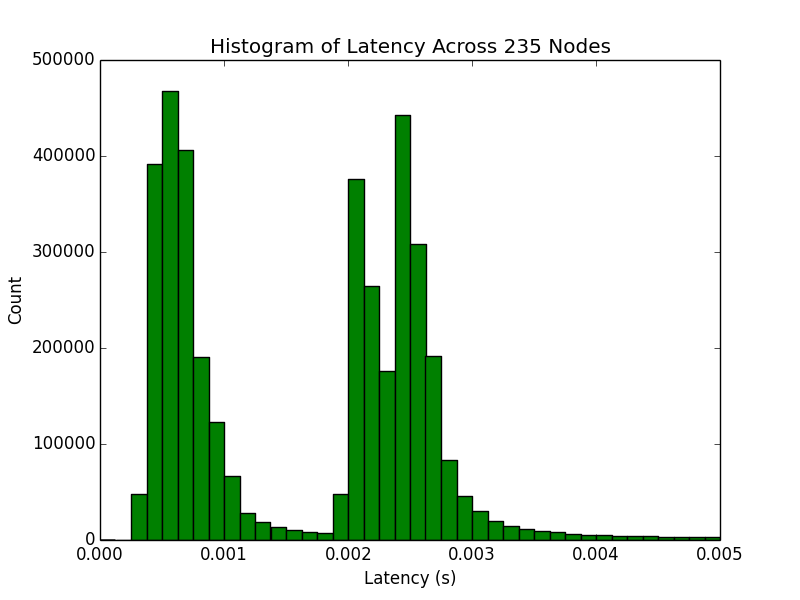
\includegraphics[width=0.8\textwidth]{latency-hist.png}
\end{figure}

\begin{figure}[!htbp]
  \centering
  \caption{~Histogram of NTP's frequency offset for Burnupi machines in the Ceph test cluster.
  The average frequency
  offset for individual Burnupi machines is -5.2 PPM with average
  standard deviation 1.1 PPM.}
  \label{fig:burnupi-hist}
  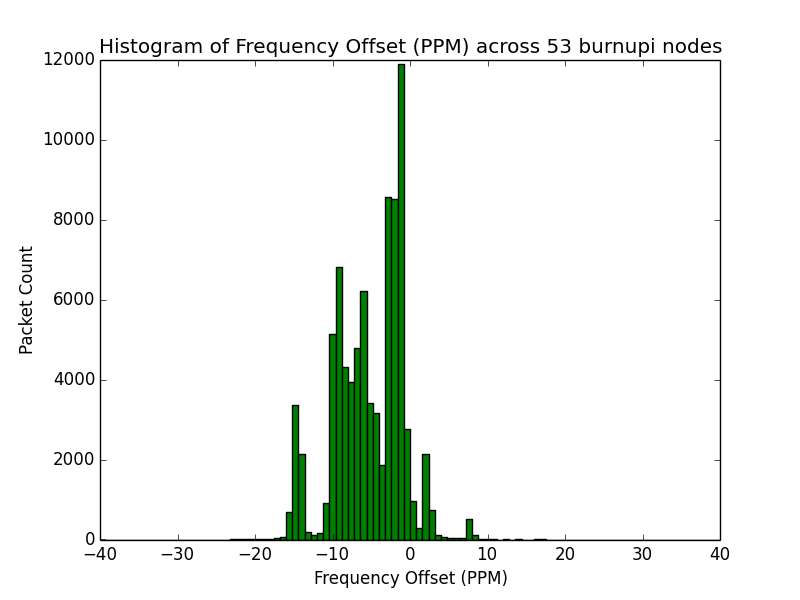
\includegraphics[width=0.8\textwidth]{burnupi-freq-offset.png}
\end{figure}

\begin{figure}[!htbp]
  \centering
  \caption{~Histogram of NTP's frequency offset for Mira machines in the Ceph test cluster.
  The average frequency offset for individual Mira machines is 10.8 PPM with average
  standard deviation 0.4 PPM.}
  \label{fig:mira-hist}
  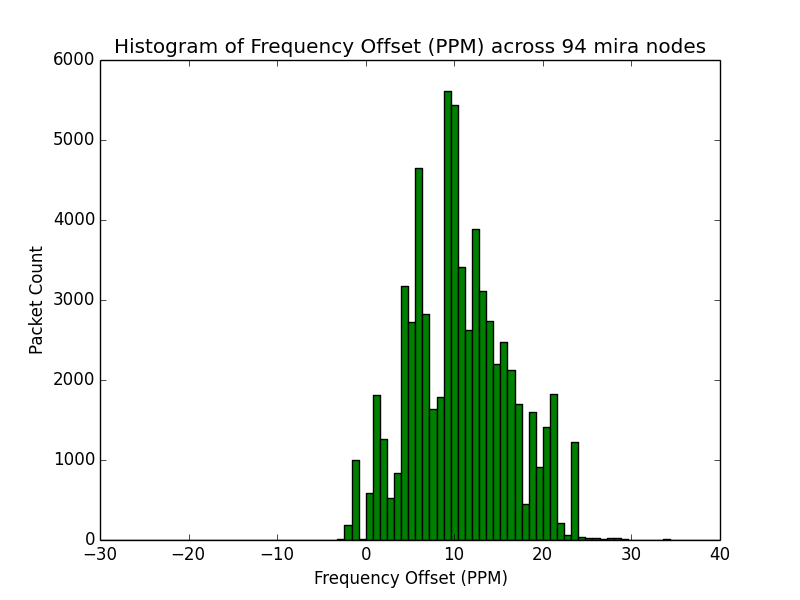
\includegraphics[width=0.8\textwidth]{mira-freq-offset.png}
\end{figure}

\begin{figure}[!htbp]
  \centering
  \caption{~Histogram of NTP's frequency offset for Plana machines in the Ceph test cluster.
  The average frequency offset for individual Plana machines is 13.3 PPM with average
  standard deviation 1.7 PPM.}
  \label{fig:plana-hist}
  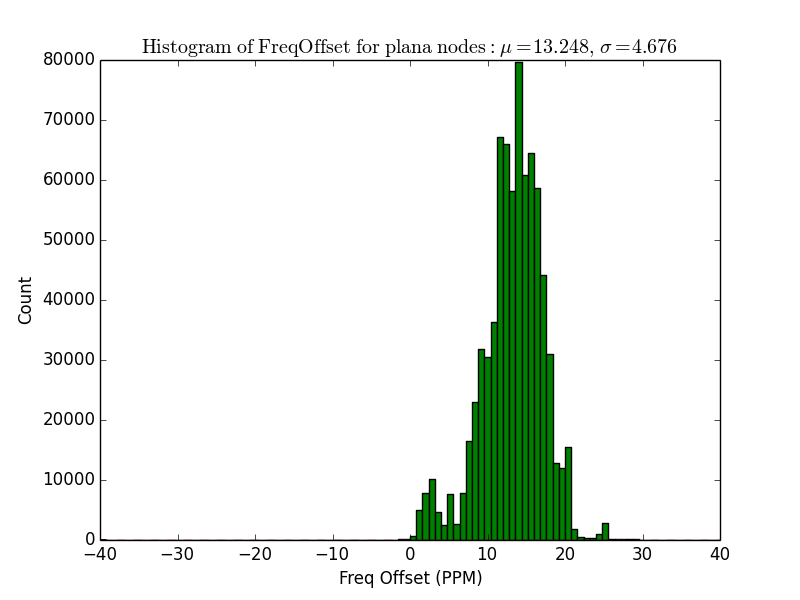
\includegraphics[width=0.8\textwidth]{plana-freq-offset.png}
\end{figure}


Figures~\ref{fig:burnupi-hist},~\ref{fig:mira-hist},
and~\ref{fig:plana-hist} show the behavior of clock frequency offset
on the three types of machines in the Ceph cluster. The distribution of frequency
offsets on all three types of machines are consistent with a 
normal distribution. The average standard deviation across all
nodes is 1.033 PPM, and the mean values of each type are reasonable as we would 
generally expect frequency offset to be at most $\pm 20$ PPM~\citep{gregscott}. 
It is interesting to note that the Burnupi
machines with the AMD chips have primarily negative clock frequency
offset, while the Mira and Plana machines with Intel chips have
primarily positive clock frequency offsets.



        



\section{Analysis of Simulation of NTP}

With the data collected on frequency offset and network latency, we
can now simulate a test cluster with input parameters that reflect the
real world. Recall that we cannot simply use a real Ceph
cluster to observe overlapping freeze windows because there is no
way to observe the real time on a given computer. A simulated network
environment running on a single computer has the advantage of having a
single clock on which all simulated clocks are based. By having a
single clock, we are able to quantify and verify the claims that time
synchronization protocols make about the quality of a synchronization
and the quality of the clocks involved.

%TODO:
% NOTE: I'm not sure this paragraph is needed?
% By using a simulation that abstracts the clock from a physical clock,
% we also eliminate any potential for idiosyncrasies of the host system
% clock to affect the measurements gathered in the simulation. This has
% the added benefit of allowing the simulation to run at a speed much
% greater than real time.
We have chosen to use an environment called
\texttt{clknetsim} %TODO reference to clknetsim repo?
to conduct our simulations. The open-source simulation package
\texttt{clknetsim} is developed and used by a major contributor to the
\texttt{chrony} project~\citep{chrony} and the \texttt{linuxptp}
project~\citep{linuxptp} to test these protocol implementations. In
comparison to commercial network simulation products, it provides a
simple codebase and feature set targeted at measuring time across a
simulated network. We have made slight additions to and modifications
of the \texttt{clknetsim} package. These extensions were made in order
to expose state parameters of NTP that were not being exposed,
including the maximum error term.

The package \texttt{clknetsim} makes use of the environment variable
\texttt{LD\_PRELOAD} in the Linux library to intercept system calls
that time sychronization libraries make on their hosts. Using these
intercepted calls, \texttt{clknetsim} is able to monitor and capture
the internal state of the synchronization program. It is also able to
fully control the information the host's time library receives from
the network and the system clock. As \texttt{clknetsim} is
manipulating system clocks and network connections for the simulation,
it can shape the behavior of the clock and network parameters to test
different setups and hardware properties.

We are most interested in measuring two parameters in this system. We
first want to determine if the uncertainty bounds reported by NTP is
correct. We can check that the uncertainty bounds report is correct
by ensuring that the uncertainty bounds on a given machine clock's
time includes the real time.  The \texttt{clknetsim} package, for a
given point-in-time in the simulation, allows us to observe what NTP
estimates the time is along with information about how certain NTP is
about that time. Our second goal is to analyze the accuracy of the
time synchronization: the magnitude of the uncertainty.  As 
CASTS is predicated on a upper bound of the uncertainty in time,
performance analysis can be accomplished by observing how modifying
parameters such as network latency affect the uncertainty bounds
that NTP reports.
%TODO: effect?

\subsection{Simulation Using Real-World Parameters}

For each node, NTP has an estimate for the real time and an uncertainty
in that estimate. \texttt{Clknetsim} allows us to access that information, and
it lets us to know the real time of the system. All of this admits
us to know what the ``safety buffer" is for each node in real time.

Recall the safety buffer first introduced in Section~\ref{sec:overlapping}, $S(t)$,  for a particular node is defined as:

\[ S(t) = U(t) - | t - E(t)| \]

where $t$ is the real time, $U(t)$ is NTP's uncertainty in the real
time estimate for that node, and E(t) is NTP's estimate for what the
real time is. In simpler terms, the safety buffer tells us where in NTP's
uncertainty range lies the error from real time (see
Figure~\ref{fig:safety-diag}). If the safety buffer is a positive
value, then the difference between NTP's estimate and real time is
within its uncertainty range. If it is negative, then its error is
outside of its uncertainty range, meaning that NTP does not function as
we would expect.

\begin{figure}[!htbp]
  \caption{~The safety buffer tells us where NTP's error in what the real time is lies within its uncertainty range.} 
  \label{fig:safety-diag}
  \centering
  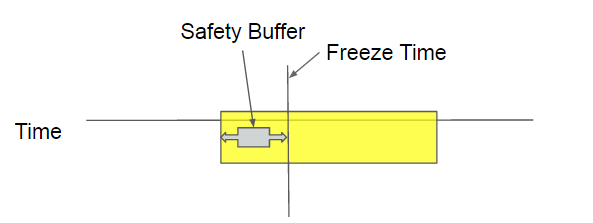
\includegraphics[width=0.5\textwidth]{safety-diagram.png}
\end{figure}

The NTP specification declares that the maximum error it reports is
the uncertainty in the time accounting for error from all
sources~\citep{Burbank2010}.  While running simulations, we monitored
the safety buffer to test if \texttt{ntpd} is implementing the
uncertainty calculation as we would expect and to quantify how much
\texttt{ntpd} overestimates the uncertainty.  When parameterizing the
simulation with latency values recorded from the Ceph cluster, we
observed safety values summarized in Figure~\ref{fig:safety-data}.

We can see that all of these values are positive. The daemon
\texttt{ntpd} does seem to function as expected under the simulation
conditions we observed.

\begin{figure}[!htbp]
  \caption{~Generated from uncertainty data recorded during simulation paramaterized
  with latencies recorded during monitoring of Ceph cluster. Uncertainty and time
  data was recorded once per second in the simulation and the included statistics 
  generated from the total dataset after the simulation was allowed to stabilize. 
  The positive values indicate that the real time is occurring within \texttt{ntpd}'s 
  uncertainty interval.}
  \label{fig:safety-data}
  \centering
  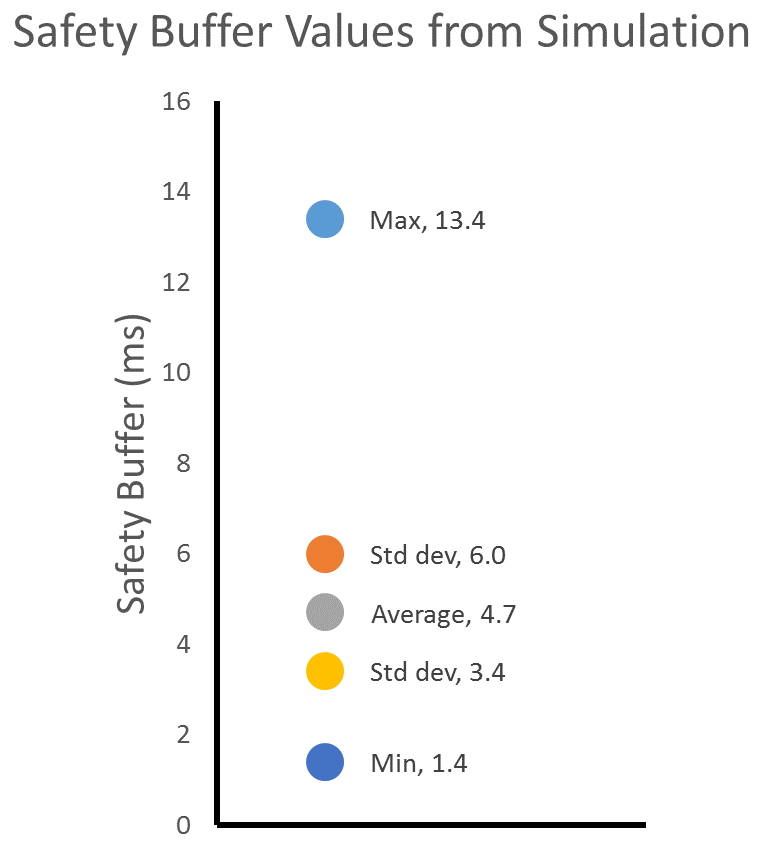
\includegraphics[width=0.55\textwidth]{5pointsSafety.png}
\end{figure}

\subsection{Generalization of Simulation Parameters}

The previous section demonstrated that \texttt{ntpd} functions as we expect in 
a real world scenario.  This section
analyzes \texttt{ntpd}'s performance under a wide variety of simulated
conditions---a wider range of conditions than \texttt{ntpd} would
likely encounter in the real world.  We found that network latency was the 
largest contributer to the uncertainty, though the relationship does not 
continue for ultra-low latency networks.

For these simulations, network latency was modeled using a gamma
distribution,
%TODO: find a citation for this?
since the data from the test Ceph cluster suggests that
latency approximately followed such a model. We varied two parameters:
the mean value and the shaping parameter, or alpha. The shaping parameter 
determines the length of the tail for the distribution: a larger value 
shortens the tail of the gamma
distribution.  A very small shaping parameter value approximates an
exponential distribution and a very large shaping parameter value
approximates a normal distribution.

%% TODO please \ref these somewhere

%% TODO: once we finalize the graphs, we should add some commentary about 
%%       the values we're seeing actually mean.
\begin{figure}[!htbp]
  \caption{~NTP's max uncertainty is plotted vs. the network latency mean and the network latency alpha parameter. We can see that the latency mean has a significant impact on the uncertainty, whereas the alpha parameter only impacts the uncertainty for large latency mean values.}
  \label{fig:max-uncertainty_latency-mean_latency-alpha}
  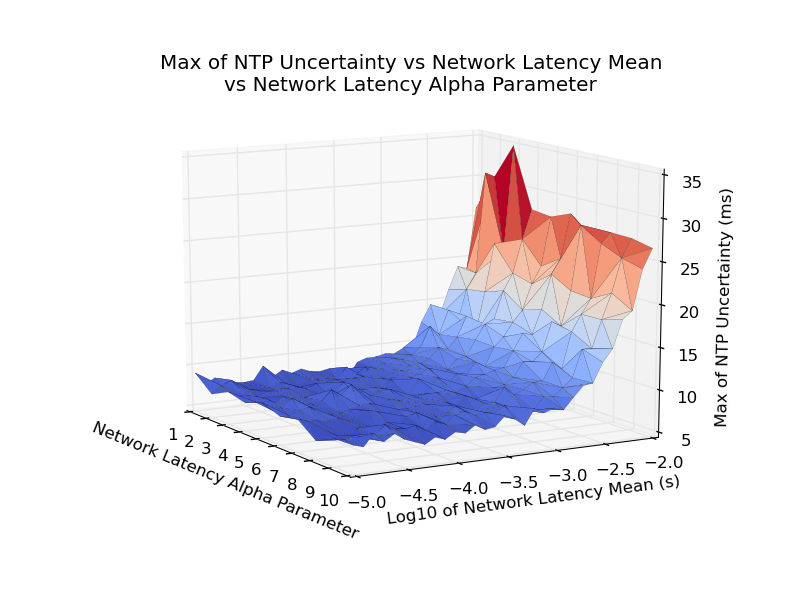
\includegraphics[width=0.8\linewidth]{max_error-latency_mean-latency_alpha.png}

  \caption{~NTP's mean uncertainty is plotted vs. the network latency mean and the network latency alpha parameter.}
  \label{fig:mean-uncertainty_latency-mean_latency-alpha}
  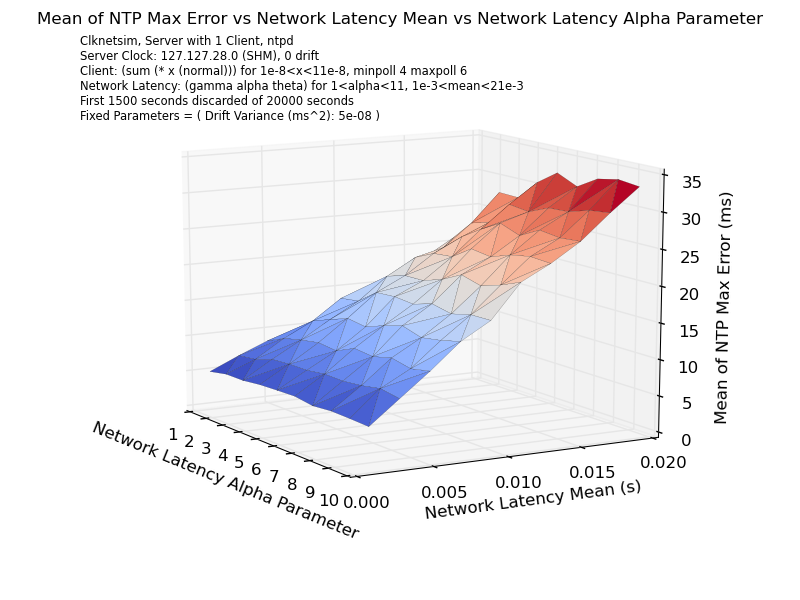
\includegraphics[width=0.8\linewidth]{mean_max_error-mean_latency-latency_alpha.png}  
\end{figure}
%% Put in the appendix
% \begin{figure}[h]
%   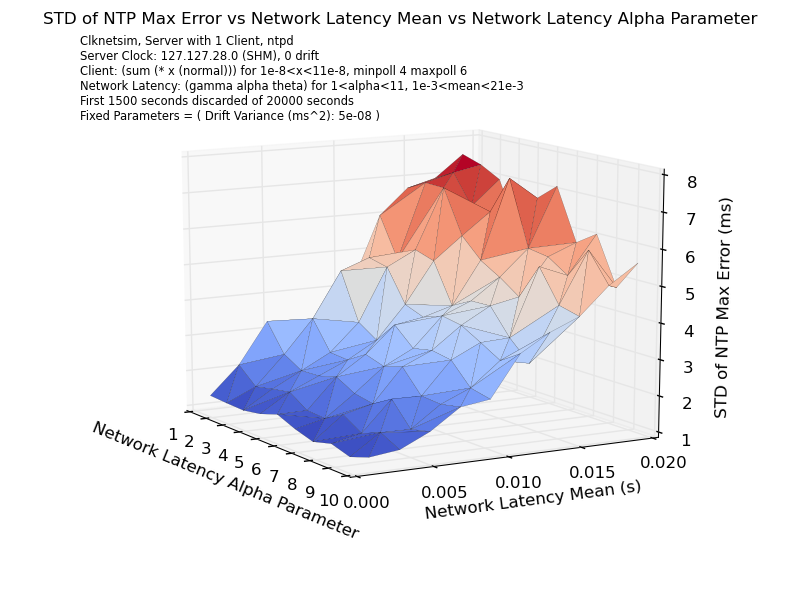
\includegraphics[width=0.8\linewidth]{max_err_stddev-latency_mean-latency_alpha.png}
% \end{figure}

%% TODO: once we finalize the graphs, we should add some commentary about 
%%       the values we're seeing actually mean.

The maximum uncertainty value observed during a simulation is strongly
affected by the mean network latency. The shape of the latency
distribution has a much weaker effect on the maximum uncertainty
value. A low mean result in a low maximum uncertainty regardless of
the shaping parameter value. A larger shaping parameter value does
have a small effect on the maximum uncertainty. We can see this effect
in Figure~\ref{fig:max-uncertainty_latency-mean_latency-alpha} at the
top right corner.

Interestingly, we see, in Figure~\ref{fig:mean-uncertainty_latency-mean_latency-alpha}, that the mean of the measured uncertainty values
increases with increasing alpha. As alpha increases the distribution of 
latency values is more normal, resulting in more spread out latency values.
When the network
latency distribution has a long tail, most of our latency values will be less
than or below the mean value. Values larger and farther away from the
mean happen less frequently. NTP uses
filtering and prediction algorithms to improve its estimates of the
time~\citep{Burbank2010}. NTP's filtering algorithms likely catch
these anomalous values and ignores them, keeping its uncertainty at a
lower, more reasonable value. We then see lower uncertainty values for
lower alpha values.

\begin{figure}[!htbp]
  \caption{~NTP's mean uncertainty is plotted vs. the network latency mean and the clock's drift variance. We can see that, compared to the latency mean, the clock drift variance has very little impact on the uncertainty.}
  \label{fig:max-uncertainty_latency-mean_drift-variance}
  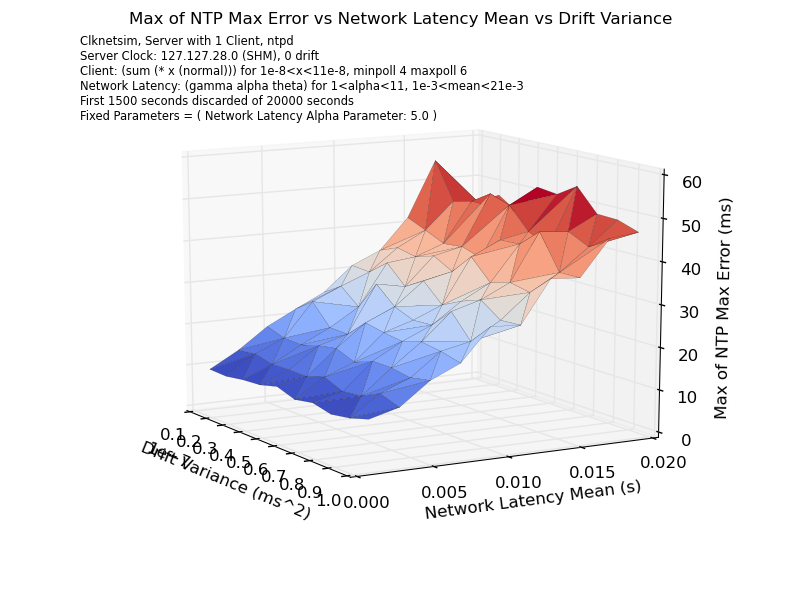
\includegraphics[width=0.8\linewidth]{max_max_err-mean_latency-drift_variance.png}

  \caption{~NTP's max uncertainty is plotted vs. the network latency mean and the clock's drift variance.}
  \label{fig:mean-uncertainty_latency-mean_drift-variance}
  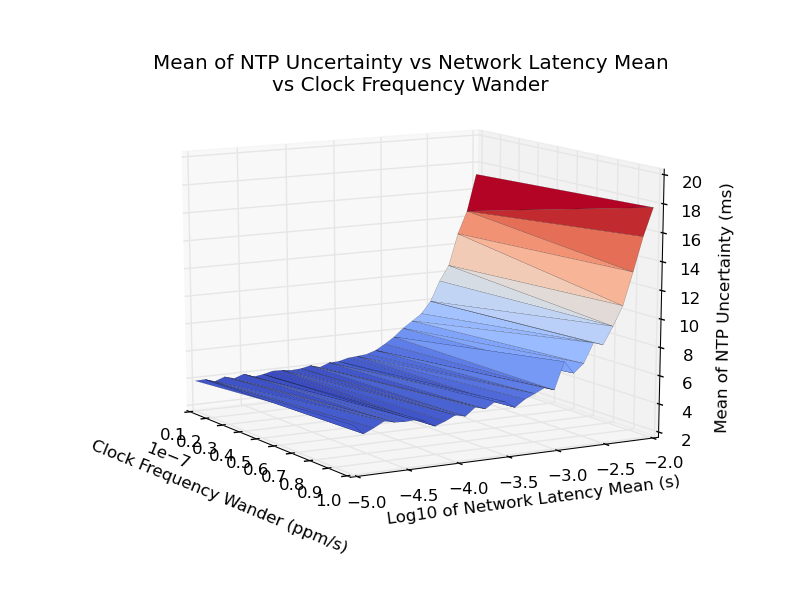
\includegraphics[width=0.8\linewidth]{mean_max_err-mean_latency-drift_variance.png}
\end{figure}

Figure~\ref{fig:max-uncertainty_latency-mean_drift-variance} and
Figure~\ref{fig:mean-uncertainty_latency-mean_drift-variance} show how
clock frequency variation, or clock wander, affects the size of the
uncertainty value.  We can see that there is very little, if any,
effect from a clock's wander on the maximum uncertainty term. The
slope along the x-axis (clock frequency wander) is effectively 0, a
horizontal line. This is expected: network latency is a term with a
much larger magnitude than the wander of even the worst clocks. We do
see a linear correlation between mean latency and the uncertainty term.

In each of these graphs, there is a clear floor: the mean of the
measured uncertainty values does not drop below four
milliseconds, even when the latency mean is tens of microseconds. 
This suggests that NTP will work well in scenarios
involving commodity network hardware where latencies are not necessarily ultra-
low. However, in ultra-low latency scenarios, it may be advantageous to look 
for a protocol that is designed more specifically for a high performance 
network.



%% Put in the appendix
% \begin{figure}[t]
%   \caption{}
%   \label{fig:stddev-mean-drift-var}
%   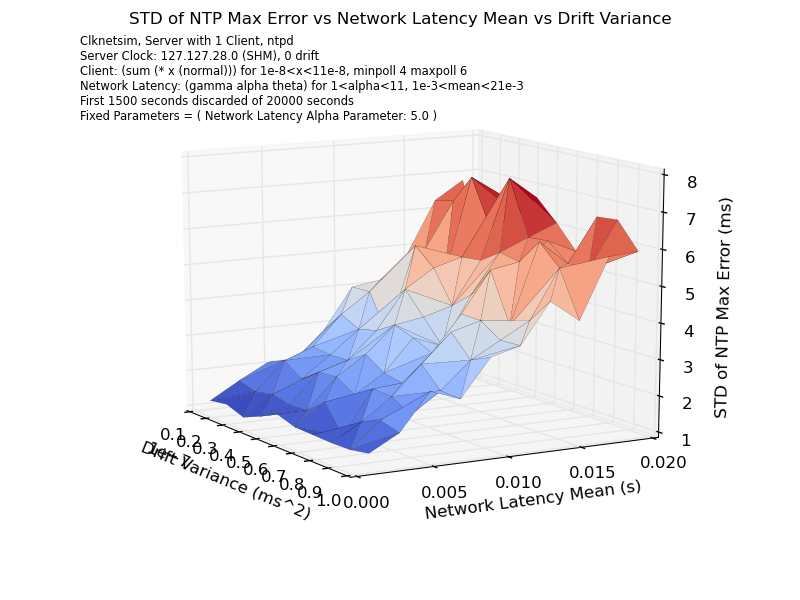
\includegraphics[width=0.8\linewidth]{stddev_max_err-mean_latency-drift_variance}
% \end{figure}

%% Put these figures in an appendix
% \begin{figure}[h]
%   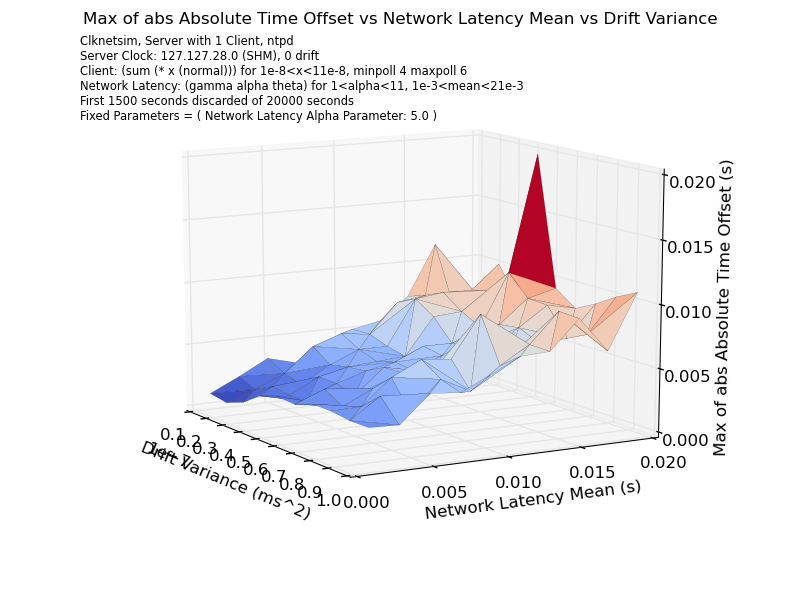
\includegraphics[width=0.8\linewidth]{max_abs_time-latency_mean-drift_var.png}
% \end{figure}

% \begin{figure}[h]
%   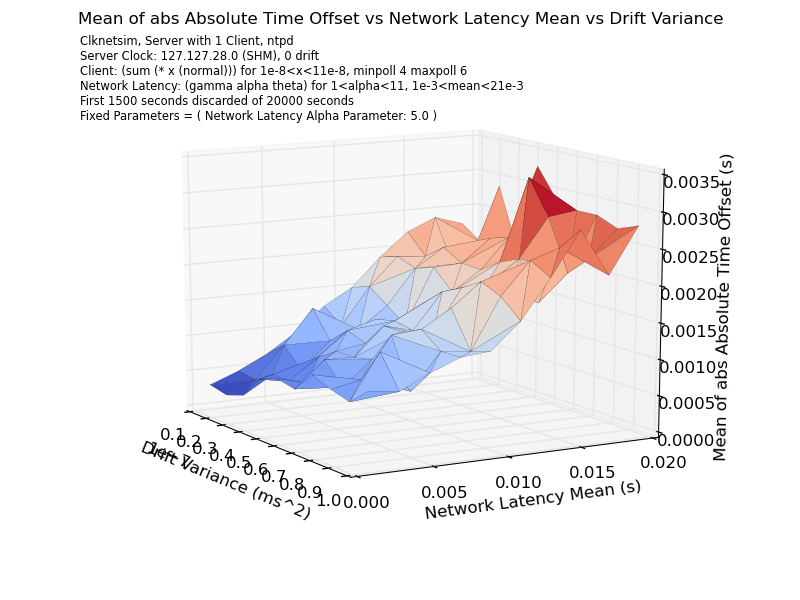
\includegraphics[width=0.8\linewidth]{mean_abs_time-mean_latency-drift_var.png}
% \end{figure}


%% Put these figures in an appendix
% \begin{figure}[h]
%   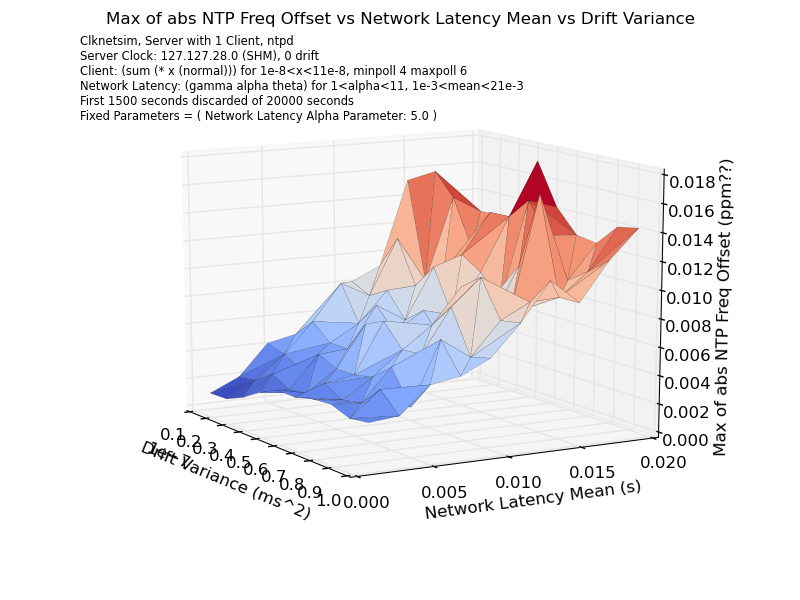
\includegraphics[width=0.8\linewidth]{max_abs_freq-mean_latency-drift_var.png}
% \end{figure}

% \begin{figure}[h]
%   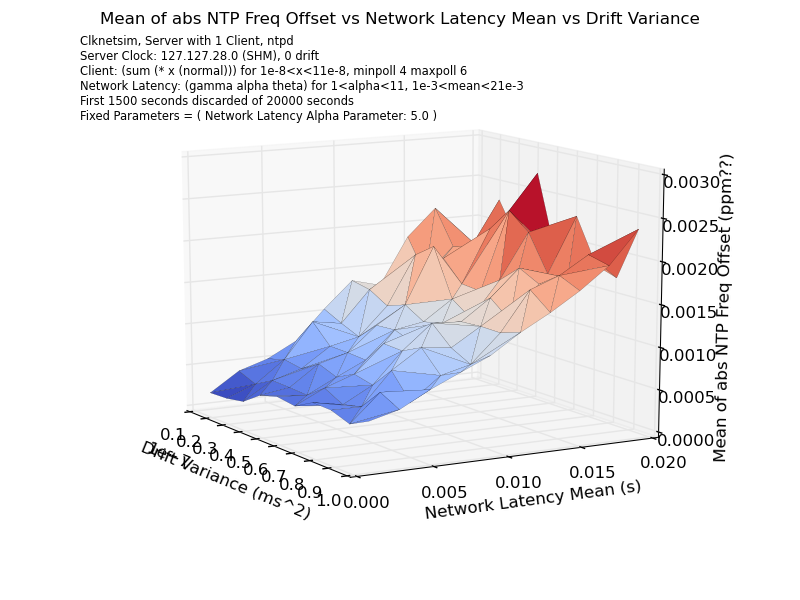
\includegraphics[width=0.8\linewidth]{mean_abs_freq-mean_latency-drift_var.png}
% \end{figure}

% \begin{figure}[h]
%   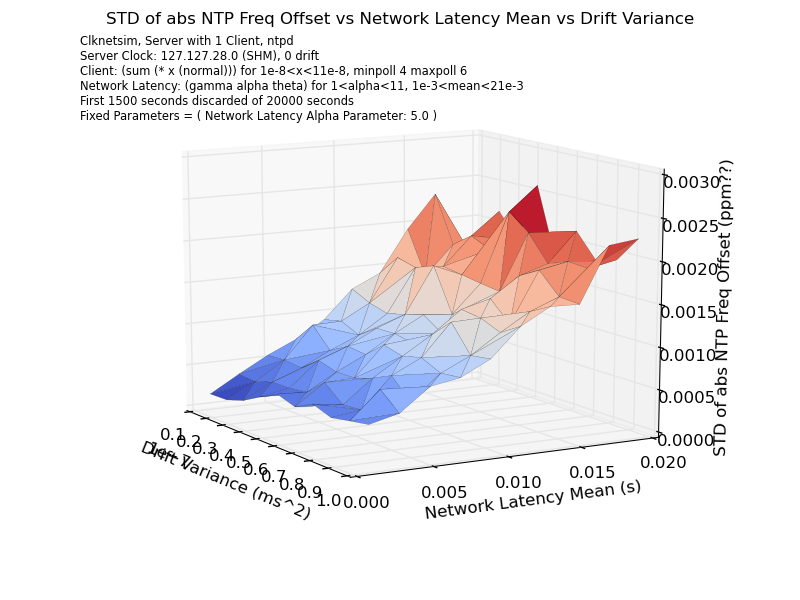
\includegraphics[width=0.8\linewidth]{stddev_abs_freq-mean_latency-drift_var.png}
% \end{figure}

% For larger variance in the drift, NTP does have to make larger
% frequency corrections, but it seems that NTP is more than capable of
% doing this, as these clock discipline corrections do not seem to
% translate into larger error or larger absolute time offsets. As the
% mean latency increases, NTP also seems to make larger frequency
% corrections. This likely means that, due to network asymmetries, NTP
% is more likely to over-correct or under-correct at times, resulting in
% an increase in the maximum offset. We also see that more normal
% latency distributions also result is smaller deviations in the
% frequency offset. The mean seems to not be significantly affected by
% either the latency or the drift variance, suggesting that most of the
% the clock frequency changes are the result of overcorrection and not
% the result of the clock actually keeping poor time. For graphs describing the 
% frequency offset values, see the appendix.

%% TODO: figure out which appendix this is going to be ^^

In summary, network latency mean has a large effect on the length of freeze 
windows. Latency value distribution does have an effect on freeze times, but
its effect is small in comparison to mean network latency. An
individual node's clock's drift variance is inconsequential to the
final performance of CASTS.

Uncertainties compound in NTP, thus it is advisable to acquire a
single, perfect clock to serve as a master. This will significantly
decrease the length of freeze windows.


